\documentclass{beamer}

\mode<presentation> {
  \usetheme{Boadilla}
    \usecolortheme{whale}

  \setbeamercovered{transparent}
}

\usepackage[spanish]{babel}
\usepackage[utf8]{inputenc}
\usepackage{pdfpages}
\usepackage{alltt}
\usepackage{verbatim}
\usepackage{hyperref}

\title[Métodos Numéricos II]
{Método de Romberg}

\author[MAC]{Diego Hernández Landeros\\ \and Ana Karen Murillo \\\and Fernanda Ibarra \\\and Daniel Escalante\\
\\$\,$\\
\centering

\includegraphics[width=2cm]{mac.png}
}

\institute[]{
UNAM-FES Acatlán, Matemáticas Aplicadas y Computación}

% Delete this, if you do not want the table of contents to pop up at
% the beginning of each subsection:

\AtBeginSubsection[]
{
  \begin{frame}<beamer>{Contenido}
    \tableofcontents[currentsection,currentsubsection]
  \end{frame}
}


% If you wish to uncover everything in a step-wise fashion, uncomment
% the following command: 
%\beamerdefaultoverlayspecification{<+->}

\begin{document}

\begin{frame}
  \titlepage
\end{frame}

%%%%%%%%%%%%%%%%%%%%%%%%%%%%%%%%%%%%%%%%%%%%%%%%%%
\section{Introducción}
\subsection{¿Qué es?}

\begin{frame}{¿Qué es?}
La integración de Romberg es una \alert{técnica} de diseño para obtener integrales numéricas \alert{(aproximaciones)} de funciones de manera eficiente, que se basa en aplicaciones sucesivas de \alert{la regla del trapecio}. Sin embargo a través de las manipulaciones matemáticas, se alcanzan mejores resultados con menos trabajo.\\
\\$\,$\\ %SALTO DE LINEA

\end{frame}

%%%%%%%%%%%%%%%%%%%%%%%%%%%%%%%%%%%%%%%%%%%%%%%%%%
\subsection{¿Cuándo se utiliza?}
    \begin{frame}{¿Cuándo se utiliza?}
El problema en la práctica se presenta cuando nos vemos imposibilitados a encontrar la
función primitiva requerida, aún para integrales aparentemente sencillas como\\
{\small \[I=\int_{0}^{1}e^{x^{2}}\]}
la cual simplemente es imposible de resolver con el Teorema Fundamental del Cálculo y resolveremos más adelante.
\\$\,$\\
El algoritmo de Romberg forma parte de una técnica conocida como método de extrapolación de Richardson.
\end{frame}

%%%%%%%%%%%%%%%%%%%%%%%%%%%%%%%%%%%%%%%%%%%%%%%%%%
\subsection{Regla del trapecio}
    \begin{frame}{Fórmula}
Para realizar el método de Romberg se usa la fórmula del trapecio.
\begin{alertblock} 
    {\centering\bf Fórmula del trapecio}
        \[A\approx\frac{\triangle x}{2}\,\left(f_{x_{0}}+f_{x_{n}}\right)\,+\,2\sum\, resto\, de\, las\, ordenadas\]\\
        \\
        {$h=\frac{b-a}{2}$}\\
        a=límite inferior\\
        b=límite superior\\
        n=subintervalos(número de trapecios en el método)\\
        $f_{x_{0}}$=primer valor\\
        $f_{x_{n}}$=último valor\\
        $\sum$=suma de los valores que están dentro del intervalo
        \end{alertblock}
\end{frame}

%%%%%%%%%%%%%%%%%%%%%%%%%%%%%%%%%%%%%%%%%%%%%%%%%%
\section{Desarrollo}
  \subsection{¿Qué se hace?}
        \begin{frame}{¿Qué se hace?}
Consiste en ir haciendo segmentos y entre más pequeños sean nuestros segmentos, más iremos aproximando al área de una función.
  \begin{alertblock}{\centering \bf Lo que se va obteniendo de cada aproximación con Romberg} 
	\begin{center}
		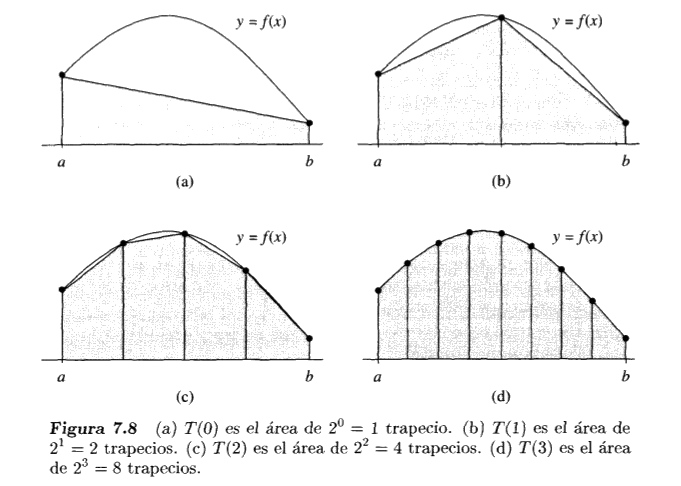
\includegraphics[height=4cm]{fig1.png}\footnote{Burden}\\
    \end{center}
\end{alertblock}
\end{frame}

%%%%%%%%%%%%%%%%%%%%%%%%%%%%%%%%%%%%%%%%%%%%%%%%%%
        \begin{frame}{¿Qué se hace?}
  \begin{center} 
    {\LARGE Finalizado el ejercicio se hará un ejemplo más gráfico usando Geogebra}\\
  \end{center}

\end{frame}
\end{frame}

%%%%%%%%%%%%%%%%%%%%%%%%%%%%%%%%%%%%%%%%%%%%%%%%%%
\subsection{Ejemplo}
\begin{frame}{Ejemplo}
\begin{exampleblock}
	{\centering\bf{Función a integrar numéricamente}}
Se nos da la siguiente función para resolver por el método de Romberg.
\begin{center}
\alert{{\huge \[\int_{0}^{1}e^{x^{2}}dx\]}}\\
\alert{{\LARGE $n=1,2,4$}}\\
\par\end{center}
\end{exampleblock} 
\end{frame}


%%%%%%%%%%%%%%%%%%%%%%%%%%%%%%%%%%%%%%%%%%%%%%%%%%
\begin{frame}{Ejemplo}
El método se va haciendo por niveles y para sacar el primer nivel necesitamos aplicar directamente la fórmula del trapecio.\n
	\begin{center}
		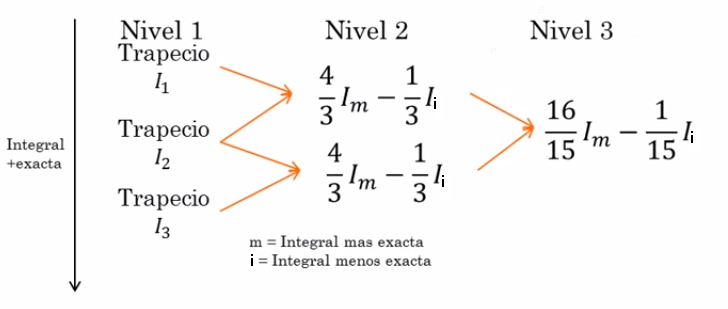
\includegraphics[height=4cm]{tabla.png}
    \end{center}
\end{frame}

%%%%%%%%%%%%%%%%%%%%%%%%%%%%%%%%%%%%%%%%%%%%%%%%%%
\begin{frame}{Ejemplo}
\begin{alertblock} 
    {\centering\bf Coeficientes del nivel requerido}
Para un nivel \textit{\textbf{2, 3, ..., n}} ya se tienen ciertas fórmulas. Los coeficientes irán variando dependiendo del nivel y la fórmula para calcular los coeficientes es: \\
\begin{center}
\huge{$\frac{4^{k-1}}{4^{k-1}-1}l_{m}-\frac{1}{4^{k-1}-1}l_{l}$}
\\$\,$\\
{\small $l_{m}=integral\, más\, exacta$}\\
{\small $l_{l}=integral\, menos\, exacta$}
\par\end{center}
\end{alertblock}
\end{frame}

%%%%%%%%%%%%%%%%%%%%%%%%%%%%%%%%%%%%%%%%%%%%%%%%%%
\begin{frame}{Calculando Nivel 1 $l_{1}$}
Para \alert{n=1} se calcula con la fórmula del trapecio de un segmento 
\begin{center}
\alert{{\small A\approx\frac{h}{2}\left[f(b)+f(a)\right]]}}
\par\end{center}
\\$\,$\\
% You can reveal the parts of a slide one at a time
% with the \pause command:
\begin{columns}
\column{0.5\textwidth}
Teniendo lo valores
\\$\,$\\
\alert{$a=0; b=1; h=\frac{b-a}{n}$}
\\$\,$\\ 
... sustituyendo
\\$\,$\\
\alert{$A\approx\frac{1}{2}\left[1+2.718282\right]$}

\column{0.5\textwidth}
\begin{tabular}{|c|c|}
\hline 
$x$ & $f(x)$\tabularnewline
\hline 
\hline 
$0$ & $1$\tabularnewline
\hline 
$1$ & $2.718282$\tabularnewline
\hline 
\end{tabular}
\\$\,$\\
\begin{LARGE}
\begin{center}
\color{green} $l_{1}=1.859141$
\par\end{center}
\end{LARGE}
\end{columns} 
\end{frame}


\end{frame}
    
%%%%%%%%%%%%%%%%%%%%%%%%%%%%%%%%%%%%%%%%%%%%%%%%%%
\begin{frame}{Calculando Nivel 2 $l_{2}$}
Ahora \alert{n=2} se calcula de nuevo con la fórmula del trapecio 
\begin{center}
\alert{\large $A\approx\frac{h}{2}\left[f(b)+f(a)+2\left[\sum_{i=1}^{n-1}f(x_{i})\right]\right]$}
\par\end{center}
\begin{center}
\par\end{center}
\\$\,$\\
% You can reveal the parts of a slide one at a time
% with the \pause command:
\begin{columns}
\column{0.5\textwidth}
Teniendo lo valores
\\$\,$\\
\alert{$a=0; b=1; h=\frac{b-a}{n}$}
\\$\,$\\ 
... sustituyendo
\\$\,$\\
\alert{$A\approx\frac{1}{4}\left[1+2.718282+2e^{(\frac{1}{2})^{2}}\right]$}

\column{0.5\textwidth}
\begin{tabular}{|c|c|}
\hline 
$x$ & $f(x)$\tabularnewline
\hline 
\hline 
$0$ & $1$\tabularnewline
\hline 
$0.5$ & $1.284025$\tabularnewline
\hline
$1$ & $2.718282$\tabularnewline
\hline 
\end{tabular}
\begin{LARGE}
\begin{center}
\color{green} $l_{2}=1.57583$
\par\end{center}
\end{LARGE}
\end{columns} 
\end{frame}


\end{frame}

%%%%%%%%%%%%%%%%%%%%%%%%%%%%%%%%%%%%%%%%%%%%%%%%%%
\begin{frame}{Calculando Nivel 3 $l_{3}$}
Ahora con \alert{n=4}
\\$\,$\\
\begin{columns}
\column{0.5\textwidth}
Tabulando los valores tenemos:
\\$\,$\\
\begin{tabular}{|c|c|}
\hline 
$x$ & $f(x)$\tabularnewline
\hline 
\hline 
$0$ & $1$\tabularnewline
\hline 
$\frac{1}{4}$ & $1.064494$\tabularnewline
\hline 
$\frac{1}{2}$ & $1.284025$\tabularnewline
\hline 
$\frac{3}{4}$ & $1.755055$\tabularnewline
\hline 
$1$ & $2.718282$\tabularnewline
\hline 
\end{tabular}
\begin{LARGE}
\begin{center}
\par\end{center}
\end{LARGE}

\column{0.5\textwidth}
Haciendo la suma
$\sum=1.064494+1.284025+1.755055$
$=4.103574$

\\$\,$\\
... sustituyendo
\\$\,$\\
\alert{$A\approx\frac{1}{8}\left[1+2.718282+2({4.103574})$)\right}
\begin{LARGE}
\begin{center}
\color{green} $l_{3}=1.490679$
\par\end{center}
\end{LARGE}
\end{columns} 
\end{frame}
\end{frame}

%%%%%%%%%%%%%%%%%%%%%%%%%%%%%%%%%%%%%%%%%%%%%%%%%%

\begin{frame}{Sustituyendo resultados en la tabla}
Una vez que tenemos nuestros valores de $l_{1}, l_{2}, l_{3}$, los sustituimos en la tabla del método de Romberg, como nos indica.\\

\\$\,$\\
De la integral más exacta a la menos exacta
	\begin{center}
		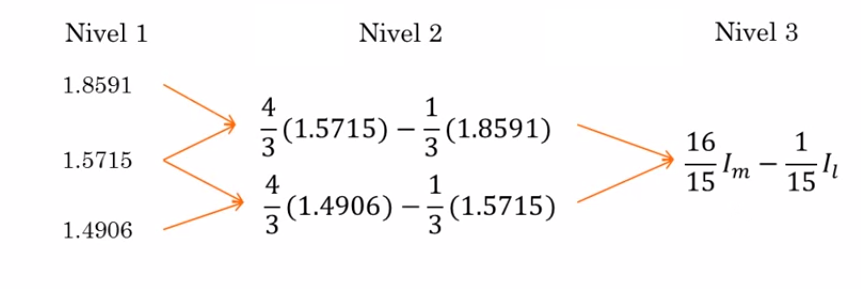
\includegraphics[height=3.5cm]{sustitucion.png}
    \end{center}
\begin{alertblock}{Los valores del nivel 1 son los valores de $l_{1}, l_{2}, l_{3}$ usando las $n$ que son los números de trapecios usados para aproximar.}
\end{alertblock}
\end{frame}
\end{frame}

%%%%%%%%%%%%%%%%%%%%%%%%%%%%%%%%%%%%%%%%%%%%%%%%%%

\begin{frame}{Evaluando todos los valores}
Evaluamos el último punto siguiendo los pasos anteriores de la integral más y menos exacta para llegar a \alert{1.4609} \\
\\$\,$\\
	\begin{center}
		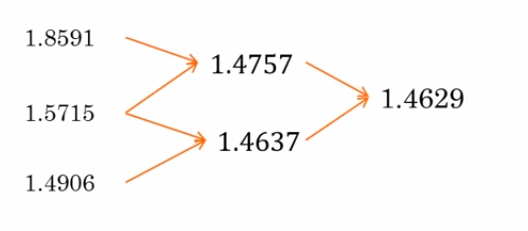
\includegraphics[height=3.5cm]{sustitucion2.png}
    \end{center}
\begin{alertblock}{En ese punto, con 3 segmentos nos aproximamos al \alert{área total} de la función en el intervalo de $0$ a $1$.}
\end{alertblock}
\end{frame}

%%%%%%%%%%%%%%%%%%%%%%%%%%%%%%%%%%%%%%%%%%%%%%%%%%
\section{Gráficos y aplicaciones}
\subsection{Wolfram}
\begin{frame}{Evaluando la función}
Metiendo la función en Wolfram da el siguiente valor...\\
\\$\,$\\
	\begin{center}
		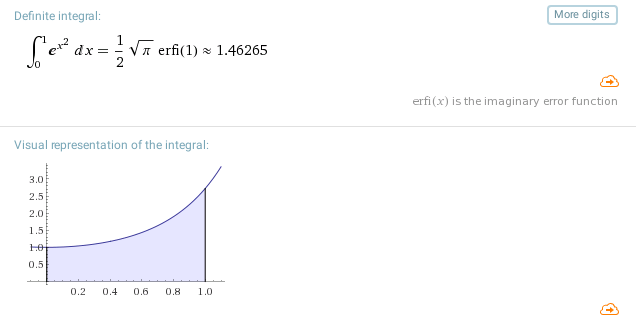
\includegraphics[height=5cm]{wolf.png}
    \end{center}
\end{frame}

%%%%%%%%%%%%%%%%%%%%%%%%%%%%%%%%%%%%%%%%%%%%%%%%%%
\subsection{Graficando}
\begin{frame}{Trapecios con Geogebra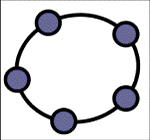
\includegraphics[height=1cm]{geoico.png}}
Usando Geogebra, se puede observar cómo es que los trapecios se van acomodando en la función conforme el valor de n se va moviendo. 
\\$\,$\\
	\begin{center}
		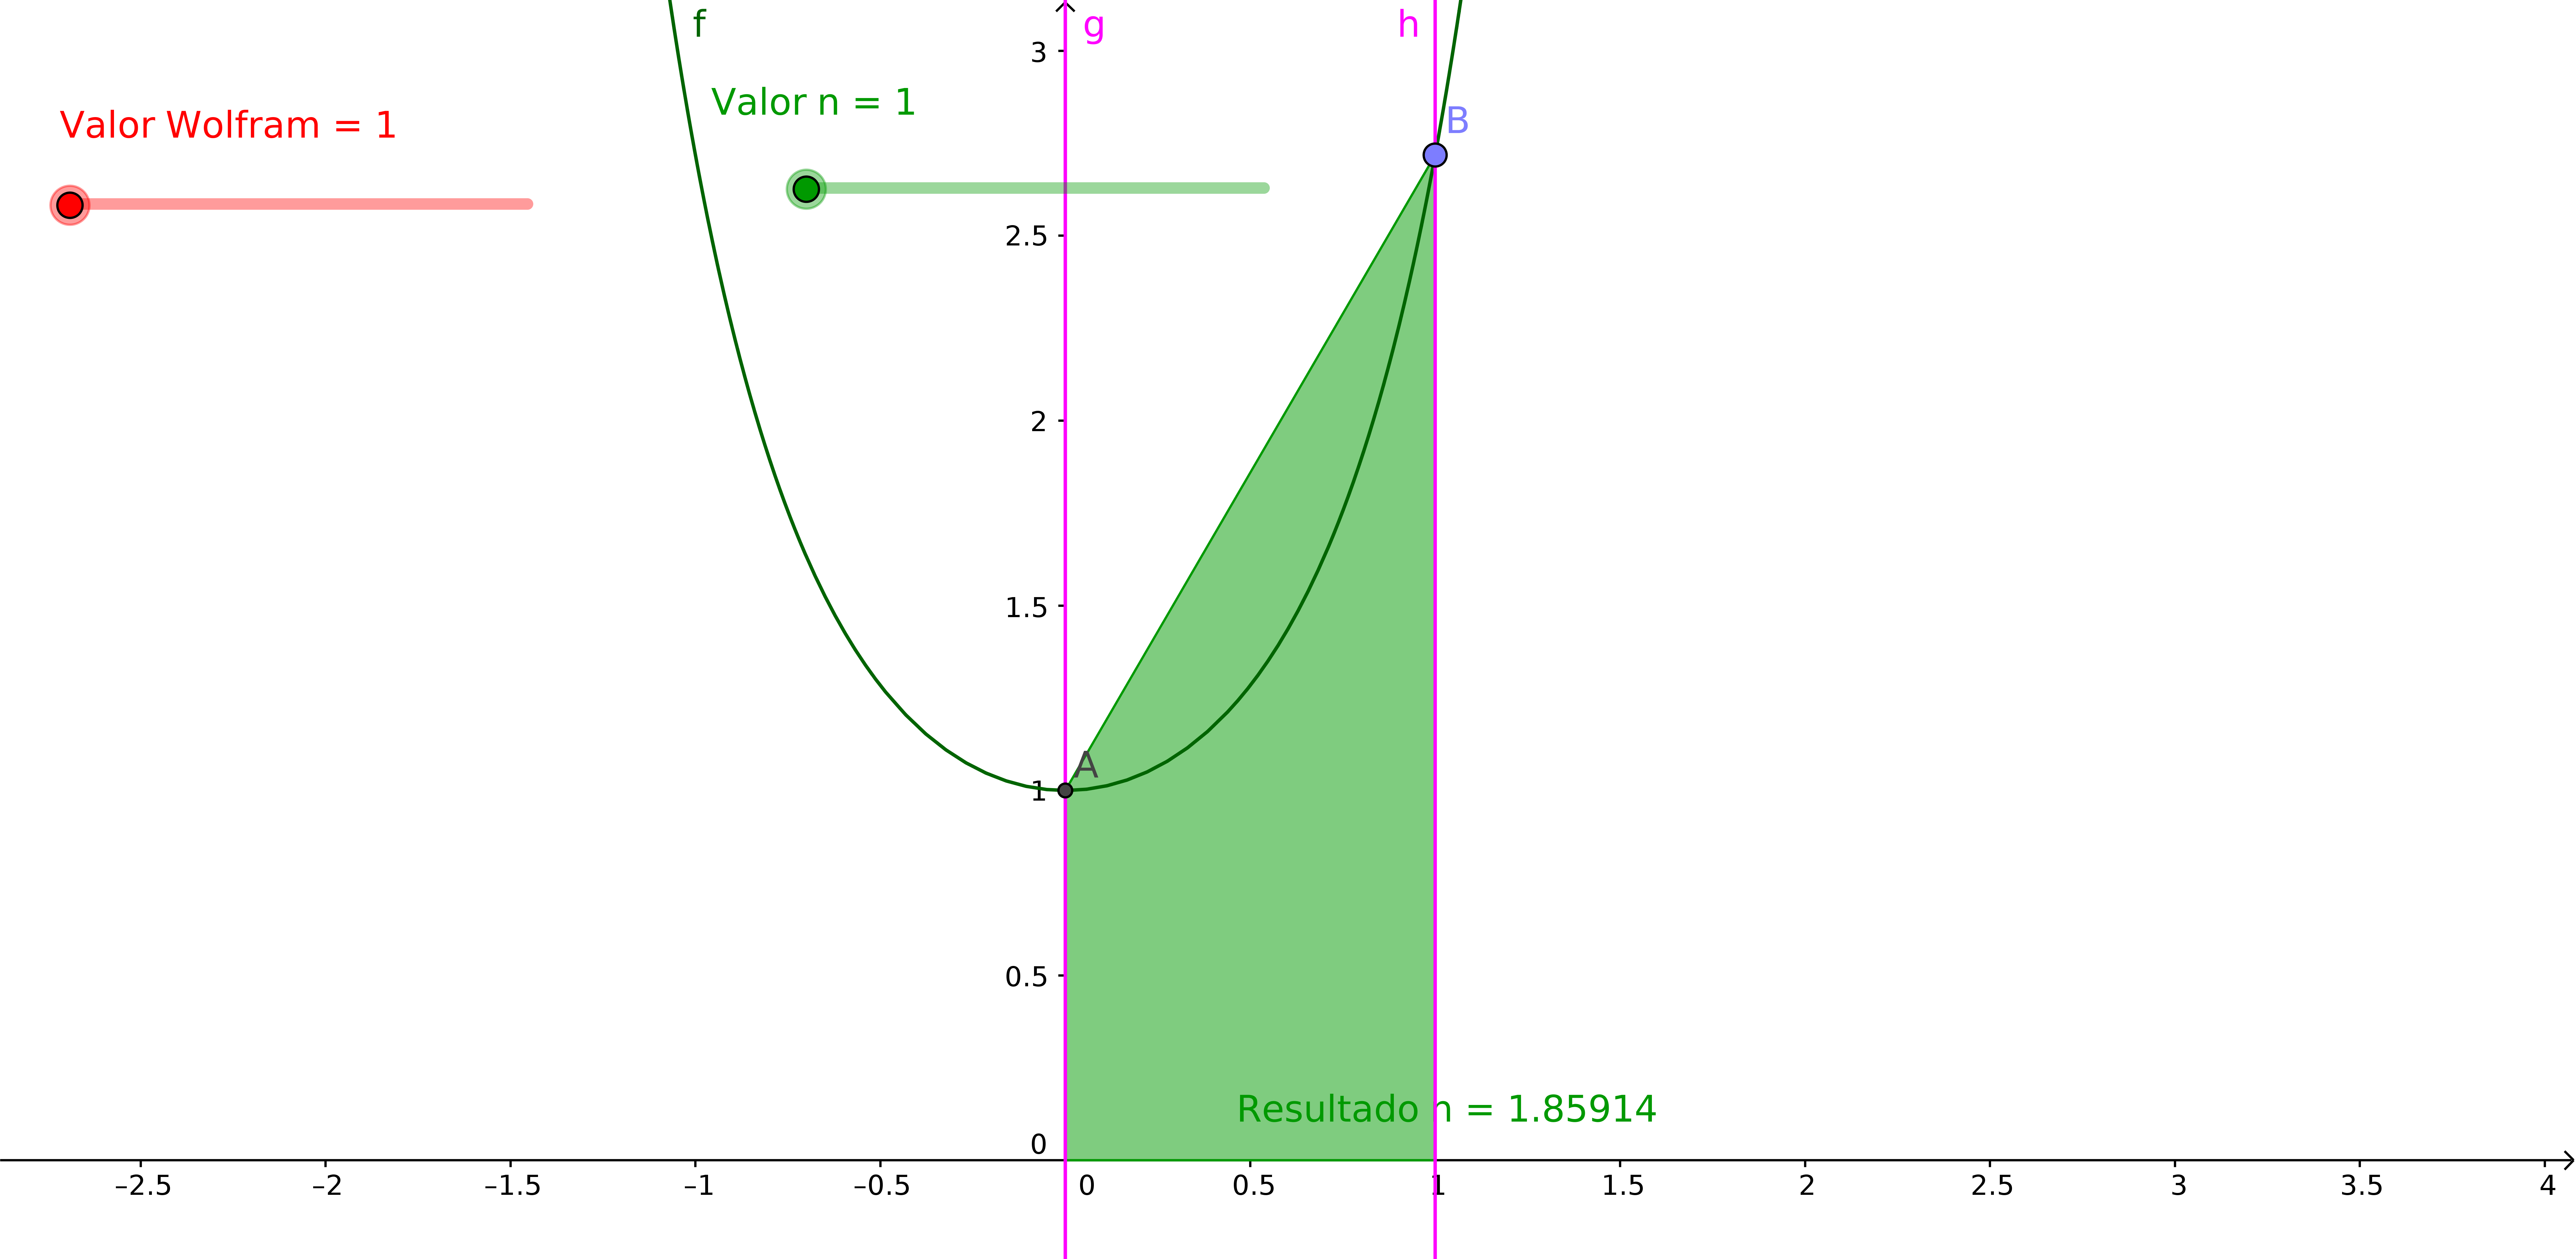
\includegraphics[height=5cm]{geo.png}
    \end{center}
\end{frame}

%%%%%%%%%%%%%%%%%%%%%%%%%%%%%%%%%%%%%%%%%%%%%%%%%%
\section{Referencias}
\appendix
\section<presentation>*{\appendixname}
\subsection<presentation>*{Fuentes}

\begin{frame}
  \frametitle<presentation>{Fuentes}
    
  \begin{thebibliography}{10}
    
  \beamertemplatebookbibitems
  % Start with overview books.

  \bibitem{}
    W. Allen Smith.
    \newblock {\em Análisis Numérico}.
    
  \bibitem{}
   Richard L. Burden
    \newblock {\em Análisis Numérico, Séptima Edición}.
    
\setbeamertemplate{bibliography item}[online]
\bibitem{A} Aproximación de áreas por el método del trapecio\\
\href{https://www.geogebra.org/material/show/id/81732}{\beamergotobutton{https://www.geogebra.org/material/show/id/81732}}
    
  \end{thebibliography}
\end{frame}


%%%%%%%%%%%%%%%%%%%%%%%%%%%%%%%%%%%%%%%%%%%%%%%%%%

\begin{frame}
\\$\,$\\
\\$\,$\\
\\$\,$\\
\\$\,$\\
\\$\,$\\

  \begin{center} 
    \Huge {¡Gracias!}\\

  \end{center}
 \\$\,$\\
 \\$\,$\\
 \\$\,$\\
 \\$\,$\\
 \\$\,$\\
 \\$\,$\\
 \\$\,$\\
 \\$\,$\\
      \begin{tiny}
(Creado con Beamer de \LaTeX) 
\end{tiny}

\end{frame}

\end{document}
